

\documentclass[../../e3_tp2_main.tex]{subfiles}

\begin{document}
\section{Ejercicio 7}


Se implementó un contador sincrónico y otro asincrónico con compuertas lógicas. Se comparó su funcionamiento y se halló la máxima velocidad de operación de cada uno.

\subsection{Contador sincronico}
Los contadores sincrónicos son aquellos que todos sus flip flop cambian de estado al mismo tiempo. Esto se debe a que cada flip clop comparte el mismo clock.
\subsubsection{Funcionamiento}
Tal como se mencionó anteriormente un contador asincrónico, basa su funcionamiento en flip flops, específicamente en flip flops tipo T.
\par El circuito lógico correspondiente al contador sincrónico de 3 bits, es el siguiente:


\begin{figure}[H]	
	\centering
	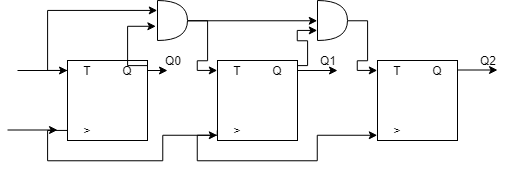
\includegraphics[width=0.5\textwidth]{imagenes/cs_b.png}
	\caption{Circuito digital contador sincronico}\label{fig:cse}
\end{figure}
El circuito de la figura \ref{fig:cse}, corresponde a un contador sincrónico de tres bits ascendente (desde cero), donde Q0 a Q2 son las salidas del contador. La entrada del circuito es un pin de enable y otro de clock.

\subsubsection{Implementación}

Se implementó el circuito previamente mencionado, con compuertas AND(74HC00) y con flip flop SR (CD4027), juntando los terminales SR se obtuvo el flip flop T.

\subsubsection{Máxima velocidad de conteo}
La máxima velocidad a la que puede contar el circuito propuesto, depende de tres factores. El tiempo de establecimiento del flip flop, el tiempo de establecimiento de la and y el tiempo de set up, tiempo que se requiere para que el sistema se estabilice.
\par De esta manera queda definido la máxima frecuencia del clock:
$$fc_{max}=\frac{1}{TeAND +TeFlipflop +TSetup   } $$

\subsection{Contador asincronico}
Los contadores asincrónicos son aquellos que la señal de clock ingresa por uno de los flip flops y se propaga por el resto.

\subsubsection{Funcionamiento}

El contador asincrónico basa su funcionamiento en flip flop T, a diferencia del contador sincronice, los flip flpos no comparten clock, sino que se conectan en cascada. 
\par El circuito lógico correspondiente es el siguiente:


\begin{figure}[H]	
	\centering
	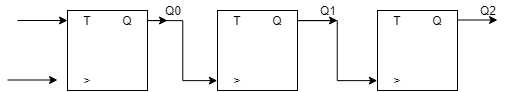
\includegraphics[width=0.5\textwidth]{imagenes/cas_b.png}
	\caption{Circuito digital contador asincronico}\label{fig:case}
\end{figure}

El circuito de la figura \ref{fig:cAse}, corresponde a un contador sincrónico de tres bits ascendente (desde cero), donde Q0 a Q2 son las salidas del contador. La entrada del circuito es un pin de enable y otro de clock.

\subsubsection{Implementación}
Se implementó el circuito anteriormente indicado, con flip flop SR (CD4027), juntando los terminales SR se obtuvo un flip flop T.

\subsubsection{Máxima velocidad de conteo}
A diferencia del contador sincrónico, el asincrónico la velocidad máxima de operación depende del tiempo de establecimiento de cada flip flop, por ende la máxima frecuencia de clock soportada es la siguiente:
$$fc_{max}=\frac{1}{N \cdot TeFlipflop } $$


\end{document}
